% An applied paper laid out the way they usually are: tables kept in their own files, notes
% under every exhibit, subfigures, an appendix that restarts the numbering, a .bib file.
\documentclass[11pt]{article}
\usepackage[margin=1in]{geometry}
\usepackage{amsmath,graphicx,booktabs,threeparttable,subcaption,multirow}
\usepackage{natbib}
\usepackage[hidelinks]{hyperref}
\usepackage{cleveref}
\crefname{table}{Table}{Tables}
\crefname{figure}{Figure}{Figures}

\begin{document}

\title{Minimum Wages and Youth Employment\thanks{We thank seminar participants for comments. All errors are ours.}}
\author{Jane Doe\thanks{University of Somewhere.} \and John Smith\thanks{Institute of Elsewhere.}}
\date{November 2026}
\maketitle

\begin{abstract}
We revisit the employment effects of state minimum wages for teenagers and young adults. Naive
panel estimates are negative; comparisons within pairs of bordering counties are close to zero.
\end{abstract}

\section{Introduction}
\label{sec:intro}

Whether minimum wages reduce employment has been debated since \citet{card1994}. Panel studies
often find losses concentrated among teenagers \citep{neumark2008}, while designs that compare
neighbouring counties do not \citep{dube2010,cengiz2019}. \Cref{tab:main} reports both for our
sample, \cref{fig:trends} shows the raw series, and \cref{tab:robust} varies the specification.

\section{Results}
\label{sec:results}

We estimate
\begin{equation}
  y_{st} = \beta \log \mathit{MW}_{st} + \alpha_s + \lambda_t + \varepsilon_{st},
  \label{eq:main}
\end{equation}
where $y_{st}$ is log employment in state $s$ and quarter $t$. The pre-period paths in
\cref{fig:trends_a,fig:trends_b} are the reason to prefer column~(2) of \cref{tab:main}.

\begin{table}[t]
\centering
\small
\setlength{\tabcolsep}{5pt}
\begin{threeparttable}
\caption{Employment Effects of the Minimum Wage}
\label{tab:main}
\begin{tabular}{@{}l@{}}\textit{Panel A: Teenagers}\end{tabular}\par\vspace{0.3em}
\begin{tabular}{@{}lccc@{}}
\toprule
 & OLS & Border pairs & Synthetic control \\
 & (1) & (2) & (3) \\
\midrule
Log minimum wage & -0.112** & -0.041 & -0.058* \\
 & (0.047) & (0.039) & (0.031) \\
\midrule
Observations & 12,240 & 6,180 & 12,240 \\
State and quarter FE & Yes & Yes & Yes \\
Pair $\times$ quarter FE & No & Yes & No \\
\bottomrule
\end{tabular}

\par\vspace{1em}
\begin{tabular}{@{}l@{}}\textit{Panel B: Young adults}\end{tabular}\par\vspace{0.3em}
\begin{tabular}{@{}lccc@{}}
\toprule
 & OLS & Border pairs & Synthetic control \\
 & (1) & (2) & (3) \\
\midrule
Log minimum wage & -0.021 & 0.006 & -0.009 \\
 & (0.018) & (0.022) & (0.015) \\
\midrule
Observations & 12,240 & 6,180 & 12,240 \\
State and quarter FE & Yes & Yes & Yes \\
Pair $\times$ quarter FE & No & Yes & No \\
\bottomrule
\end{tabular}

\begin{tablenotes}[flushleft]\footnotesize
\item \textit{Notes:} Estimates of equation~\eqref{eq:main}. Column~(2) adds county-pair by quarter effects as in \citet{dube2010}. Standard errors clustered by state. $^{*}p<0.10$, $^{**}p<0.05$.
\end{tablenotes}
\end{threeparttable}
\end{table}

\begin{figure}[t]
\centering
\begin{subfigure}{0.48\textwidth}
  \centering
  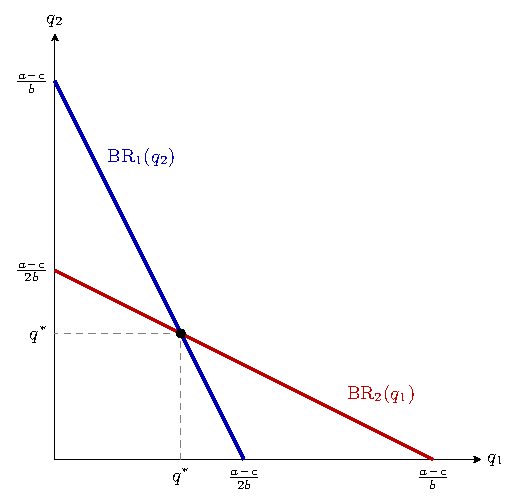
\includegraphics[width=\textwidth]{figures/reaction.pdf}
  \caption{Treated states}
  \label{fig:trends_a}
\end{subfigure}
\hfill
\begin{subfigure}{0.48\textwidth}
  \centering
  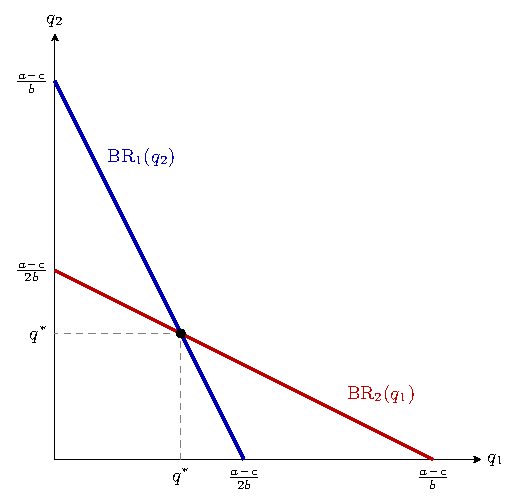
\includegraphics[width=\textwidth]{figures/reaction.pdf}
  \caption{Control states}
  \label{fig:trends_b}
\end{subfigure}
\caption{Employment Before and After the Increase}
\label{fig:trends}
\caption*{\footnotesize\textit{Notes:} Placeholder images. Each panel would plot mean log teen employment by quarter relative to the increase.}
\end{figure}

\bibliographystyle{plainnat}
\bibliography{refs}

\clearpage
\appendix
\setcounter{table}{0}
\renewcommand{\thetable}{A\arabic{table}}

\section{Additional Results}
\label{app:more}

\begin{table}[h]
\centering
\caption{Robustness of the Border-Pair Estimate}
\label{tab:robust}
\begin{tabular}{llc}
\toprule
Sample & Controls & Estimate \\
\midrule
\multirow{2}{*}{Teenagers} & None & -0.041 \\
 & Division trends & -0.036 \\
\multirow{2}{*}{Young adults} & None & 0.006 \\
 & Division trends & 0.004 \\
\bottomrule
\end{tabular}

\parbox{0.8\textwidth}{\footnotesize \textit{Notes:} Each row is a separate regression of the form in \cref{app:more}.}
\end{table}

\end{document}
